\section{ Topics covered}
\begin{itemize}

\item Agile methods

\item Plan-driven and agile development

\item Extreme programming

\item Agile project management

\item Scaling agile methods

\end{itemize}
\section{ Rapid software development}
\begin{itemize}

\item Rapid development and delivery is now often the most important requirement for software systems

\item Businesses operate in a fast –changing requirement and it is practically impossible to produce a set of stable software requirements
\item Software has to evolve quickly to reflect changing business needs.
\item Rapid software development
\item Specification, design and implementation are inter-leaved

\item System is developed as a series of versions with stakeholders involved in version evaluation
\item User interfaces are often developed using an IDE and graphical toolset.

\end{itemize}
\section{ Agile methods}
\begin{itemize}

\item Dissatisfaction with the overheads involved in software design methods of the 1980s and 1990s led to the creation of agile methods. These methods:

\item Focus on the code rather than the design

\item Are based on an iterative approach to software development

\item Are intended to deliver working software quickly and evolve this quickly to meet changing requirements.

\item The aim of agile methods is to reduce overheads in the software process (e.g. by limiting documentation) and to be able to respond quickly to changing requirements without excessive rework.


\end{itemize}
\subsection{ Agile manifesto}
\begin{itemize}

\item We are uncovering better ways of developing software by doing it and helping others do it. Through this work we have come to value:

\item Individuals and interactions over processes and tools Working software over comprehensive documentation Customer collaboration over contract negotiation Responding to change over following a plan
\item That is, whilethere is value in the items on value the items on the left more.

\end{itemize}
\subsection{The Principles of agile methods}

\begin{table}[h!]
\centering
\begin{tabular}{ |p{3cm}|p{8cm}|  }
\hline
Principles & Description  \\
\hline
Customer involvement & Customers should be closely involved throughout the development process. Their role is provide and prioritize new system requirements and to evaluate the iterations of the system.\\
\hline

Incremental delivery & The software is developed in increments with the customer specifying the requirements to be included in each increment.\\
\hline
People not process & The skills of the development team should be recognized and exploited. Team members should be left to develop their own ways of working without prescriptive processes.\\
\hline
Embrace change & Expect the system requirements to change and so design the system to accommodate these changes.\\
\hline
Maintain simplicity & Focus on simplicity in both the software being developed and in the development process. Wherever possible, actively work to eliminate complexity from the system.\\
\hline
\end{tabular}

\label{table:T1_2}
\end{table}


 \subsection{ Agile method applicability}

 \begin{itemize}
\item Product development where a software company is developing a small or medium-sized product for sale.

\item Custom system development within an organization, where there is a clear commitment from the customer to become involved in the development process and where there are not a lot of external rules and regulations that affect the software.

\item Because of their focus on small, tightly-integrated teams, there are problems in scaling agile methods to large systems.

\end{itemize}
 \subsection{ Problems with agile methods}
 \begin{itemize}


\item It can be difficult to keep the interest of customers who are involved in the process.

\item Team members may be unsuited to the intense involvement that characterises agile methods.

\item Prioritising changes can be difficult where there are multiple stakeholders.

\item Maintaining simplicity requires extra work.

\item Contracts may be a problem as with other approaches to iterative development.

\end{itemize}
\subsection{ Agile methods and software maintenance}
\begin{itemize}

\item Most organizations spend more on maintaining existing software than they do on new software development. So, if agile methods are to be successful, they have to support maintenance as well as original development.

\item Two key issues:

\item Are systems that are developed using an agile approach maintainable, given the emphasis in the development process of minimizing formal documentation?
\item Can agile methods be used effectively for evolving a system in response to customer change requests?

\item Problems may arise if original development team cannot be maintained.


\end{itemize}
 \section{ Plan-driven and agile development}
 \begin{itemize}

\item Plan-driven development

\item A plan-driven approach to software engineering is based around separate development stages with the outputs to be produced at each of these stages planned in advance.
\item Not necessarily waterfall model – plan-driven, incremental development is possible
\item Iteration occurs within activities. \item Agile development
\item Specification, design, implementation and testing are inter-leaved and the outputs from the development process are decided through a process of negotiation during the software development process.

\end{itemize}
\newpage
\section{ Plan-driven and agile specification}
\begin{figure}[h!]
    \centering
    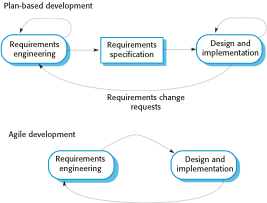
\includegraphics[width = 0.8\textwidth]{./figures/L2_1.png}
    \caption{}
    \label{fig:L2_1}
\end{figure}


 \section{ Technical, human, organizational issues}
 \begin{itemize}

\item Most projects include elements of plan-driven and agile processes. Deciding on the balance depends on:

\item Is it important to have a very detailed specification and design before moving to implementation? If so, you probably need to use a plan-driven approach.
\item Is an incremental delivery strategy, where you deliver the software to customers and get rapid feedback from them, realistic? If so, consider using agile methods.
\item How large is the system that is being developed? Agile methods are most effective when the system can be developed with a small co-located team who can communicate informally. This may not be possible for large systems that require larger development teams so a plan-driven approach may have to be used.
\item What type of system is being developed?
\newline $-$Plan-driven approaches may be required for systems that require a lot of analysis before implementation (e.g. real-time system with complex timing requirements).
\item What is the expected system lifetime?
\newline $-$Long-lifetime systems may require more design documentation to communicate the original intentions of the system developers to the support team.
\item What technologies are available to support system development?
\newline $-$Agile methods rely on good tools to keep track of an evolving design
\item How is the development team organized?
\newline $-$If the development team is distributed or if part of the development is being outsourced, then you may need to develop design documents to communicate across the development teams.

\item Are there cultural or organizational issues that may affect the system development?
\newline $-$Traditional engineering organizations have a culture of plan-based development, as this is the norm in engineering.
\item How good are the designers and programmers in the development team?
\newline $-$It is sometimes argued that agile methods require higher skill levels than plan-based approaches in which programmers simply translate a detailed design into code
\item Is the system subject to external regulation?
\newline $-$If a system has to be approved by an external regulator (e.g. the FAA approve software that is critical to the operation of an aircraft) then you will probably be required to produce detailed documentation as part of the system safety case.

\end{itemize}
\section{ Extreme programming}
\begin{itemize}

\item Perhaps the best-known and most widely used agile method.

\item Extreme Programming (XP) takes an ‘extreme’ approach to iterative development.

\item New versions may be built several times per day; \item Increments are delivered to customers every 2 weeks;
\item All tests must be run for every build and the build is only accepted if tests run successfully.

\end{itemize}

\section{ XP and agile principles}
\begin{itemize}
\item Incremental development is supported through small, frequent system releases.

\item Customer involvement means full-time customer engagement with the team.

\item People not process through pair programming, collective ownership and a process that avoids long working hours.

\item Change supported through regular system releases.

\item Maintaining simplicity through constant refactoring of code.
\end{itemize}
\section{ The extreme programming release cycle}
\begin{figure}[h!]
    \centering
    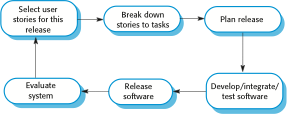
\includegraphics[width = 0.8\textwidth]{./figures/L2_2.png}
    \caption{}
    \label{fig:L2_2}
\end{figure}
\newpage
\section{ Extreme programming practices (a)}

\begin{table}[h!]
\centering
\begin{tabular}{ |p{3cm}|p{8cm}|  }
\hline
Principle or practice & Description  \\
\hline
\hline
Incremental planning & Requirements are recorded on story cards and the stories to be included in a release are determined by the time available and their relative priority. The developers break these stories into development ‘Tasks’. See Figures 3.5 and 3.6.\\
\hline
Small releases & The minimal useful set of functionality that provides business value is developed first. Releases of the system are frequent and incrementally add functionality to the first release.\\
\hline
Simple design & Enough design is carried out to meet the current requirements and no more. Test-first development \& An automated unit test framework is used to write tests for a new piece of functionality before that functionality itself is implemented.\\
\hline
Refactoring & All developers are expected to refactor the code continuously as soon as possible code improvements are found. This keeps the code simple and maintainable.\\
\hline
\end{tabular}

\label{table:T2_2}
\end{table}
\newpage
\section{ Extreme programming practices (b)}

\begin{table}[h!]
\centering
\begin{tabular}{ |p{3cm}|p{8cm}|  }
\hline
Pair programming & Developers work in pairs, checking each other’s work and providing the support to always do a good job.\\
\hline
Collective ownership & The pairs of developers work on all areas of the system, so that no islands of expertise develop and all the developers take responsibility for all of the code. Anyone can change anything.\\
\hline
Continuous integration & As soon as the work on a task is complete, it is integrated into the whole system. After any such integration, all the unit tests in the system must pass.\\
\hline
Sustainable pace & Large amounts of overtime are not considered acceptable as the net effect is often to reduce code quality and medium term productivity\\
\hline
On-site customer & A representative of the end-user of the system (the customer) should be available full time for the use of the XP team. In an extreme programming process, the customer is a member of the development team and is responsible for bringing system requirements to the team for implementation.\\
\hline
\end{tabular}

\label{table:T2_3}
\end{table}

\section{ Requirements scenarios}
\begin{itemize}

\item In XP, a customer or user is part of the XP team and is responsible for making decisions on requirements.

\item User requirements are expressed as scenarios or user stories.

\item These are written on cards and the development team break them down into implementation tasks. These tasks are the basis of schedule and cost estimates.

\item The customer chooses the stories for inclusion in the next release based on their priorities and the schedule estimates.

\end{itemize}
\section{ A ‘prescribing medication’ story}
\begin{figure}[h!]
    \centering
    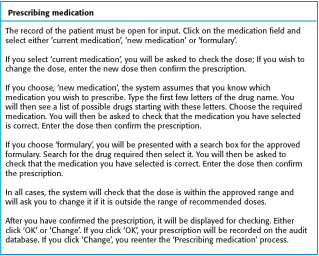
\includegraphics[width = 0.8\textwidth]{./figures/L2_4.png}
    \caption{}
    \label{fig:L2_4}
\end{figure}


\section{ Examples of task cards for prescribing medication}
\begin{figure}[h!]
    \centering
    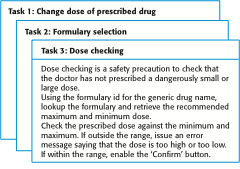
\includegraphics[width = 0.8\textwidth]{./figures/L2_5.png}
    \caption{}
    \label{fig:L2_5}
\end{figure}

\section{ XP and change}
\begin{itemize}
\item Conventional wisdom in software engineering is to design for change. It is worth spending time and effort anticipating changes as this reduces costs later in the life cycle.

\item XP, however, maintains that this is not worthwhile as changes cannot be reliably anticipated.
\item Rather, it proposes constant code improvement (refactoring) to make changes easier when they have to be implemented.
\end{itemize}

\section{ Refactoring}
\begin{itemize}

\item Programming team look for possible software improvements and make these improvements even where there is no immediate need for them.

\item This improves the understandability of the software and so reduces the need for documentation.

\item Changes are easier to make because the code is well-structured and clear.

\item However, some changes requires architecture refactoring and this is much more expensive.

\end{itemize}
\subsection{ Examples of refactoring}
\begin{itemize}

\item Re-organization of a class hierarchy to remove duplicate code.

\item Tidying up and renaming attributes and methods to make them easier to understand.

\item The replacement of inline code with calls to methods that have been included in a program library.

\end{itemize}
\section{ Key points}
\begin{itemize}

\item Agile methods are incremental development methods that focus on rapid development, frequent releases of the software, reducing process overheads and producing high-quality code. They involve the customer directly in the development process.

\item The decision on whether to use an agile or a plan-driven approach to development should depend on the type of software being developed, the capabilities of the development team and the culture of the company developing the system.

\item Extreme programming is a well-known agile method that integrates a range of good programming practices such as frequent releases of the software, continuous software improvement and customer participation in the development team.


\end{itemize}
\section{ Testing in XP}
\begin{itemize}

\item Testing is central to XP and XP has developed an approach where the program is tested after every change has been made.

\item XP testing features: \item Test-first development.
\item Incremental test development from scenarios. \item User involvement in test development and validation.
\item Automated test harnesses are used to run all component tests each time that a new release is built.

\end{itemize}
\section{ Test-first development}
\begin{itemize}

\item Writing tests before code clarifies the requirements to be implemented.

\item Tests are written as programs rather than data so that they can be executed automatically. The test includes a check that it has executed correctly.

\item Usually relies on a testing framework such as Junit.

\item All previous and new tests are run automatically when new functionality is added, thus checking that the new functionality has not introduced errors.
Customer involvement
\item The role of the customer in the testing process is to help develop acceptance tests for the stories that are to be implemented in the next release of the system.

\item The customer who is part of the team writes tests as development proceeds. All new code is therefore validated to ensure that it is what the customer needs.

\item However, people adopting the customer role have limited time available and so cannot work full-time with the development team. They may feel that providing the requirements was enough of a contribution and so may be reluctant to get involved in the testing process.


\end{itemize}
\newpage
\section{ Test case description for dose checking}
\begin{figure}[h!]
    \centering
    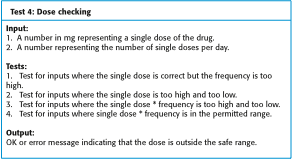
\includegraphics[width = 0.8\textwidth]{./figures/L2_6.png}
    \caption{}
    \label{fig:L2_6}
\end{figure}

\section{ Test automation}
\begin{itemize}
\item Test automation means that tests are written as executable components before the task is implemented

\item These testing components should be stand-alone, should simulate the submission of input to be tested and should check that the result meets the output specification. An automated test framework (e.g. Junit) is a system that makes it easy to write executable tests and submit a set of tests for execution.

\item As testing is automated, there is always a set of tests that can be quickly and easily executed

\item Whenever any functionality is added to the system, the tests can be run and problems that the new code has introduced can be caught immediately.


\end{itemize}
\section{ XP testing difficulties}
\begin{itemize}
\item Programmers prefer programming to testing and sometimes they take short cuts when writing tests. For example, they may write incomplete tests that do not check for all possible exceptions that may occur.

\item Some tests can be very difficult to write incrementally. For example, in a complex user interface, it is often difficult to write unit tests for the code that implements the ‘display logic’ and workflow between screens.

\item It difficult to judge the completeness of a set of tests. Although you may have a lot of system tests, your test set may not provide complete coverage.


\end{itemize}
\section{ Pair programming}
\begin{itemize}

\item In XP, programmers work in pairs, sitting together to develop code.

\item This helps develop common ownership of code and spreads knowledge across the team.

\item It serves as an informal review process as each line of code is looked at by more than 1 person.

\item It encourages refactoring as the whole team can benefit from this.

\item Measurements suggest that development productivity with pair programming is similar to that of two people working independently.

\item In pair programming, programmers sit together at the same workstation to develop the software.

\item Pairs are created dynamically so that all team members work with each other during the development process.

\item The sharing of knowledge that happens during pair programming is very important as it reduces the overall risks to a project when team members leave.

\item Pair programming is not necessarily inefficient and there is evidence that a pair working together is more efficient than 2 programmers working separately.
\end{itemize}
\subsection{Advantages of pair programming}
\begin{itemize}

\item It supports the idea of collective ownership and responsibility for the system.

\item Individuals are not held responsible for problems with the code. Instead, the team has collective responsibility for resolving these problems.

\item It acts as an informal review process because each line of code is looked at by at least two people.

\item It helps support refactoring, which is a process of software improvement.

\item Where pair programming and collective ownership are used, others benefit immediately from the refactoring so they are likely to support the process.

\end{itemize}

\section{ Agile project management}
\begin{itemize}
\item The principal responsibility of software project managers is to manage the project so that the software is delivered on time and within the planned budget for the project.

\item The standard approach to project management is plan-driven. Managers draw up a plan for the project showing what should be delivered, when it should be delivered and who will work on the development of the project deliverables.

\item Agile project management requires a different approach, which is adapted to incremental development and the particular strengths of agile methods.


\end{itemize}
\section{ Scrum}
\begin{itemize}

\item The Scrum approach is a general agile method but its focus is on managing iterative development rather than specific agile practices.

\item There are three phases in Scrum.

\item The initial phase is an outline planning phase where you establish the general objectives for the project and design the software architecture.
\item This is followed by a series of sprint cycles, where each cycle develops an increment of the system.
\item The project closure phase wraps up the project, completes required documentation such as system help frames and user manuals and assesses the lessons learned from the project.


\end{itemize}
\subsection{ The Scrum process}
\begin{figure}[h!]
    \centering
    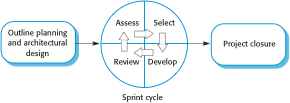
\includegraphics[width = 0.8\textwidth]{./figures/L2_7.png}
    \caption{}
    \label{fig:L2_7}
\end{figure}

\subsection{ The Sprint cycle}
\begin{itemize}

\item Sprints are fixed length, normally 2–4 weeks. They correspond to the development of a release of the system in XP.

\item The starting point for planning is the product backlog, which is the list of work to be done on the project.

\item The selection phase involves all of the project team who work with the customer to select the features and functionality to be developed during the sprint.


\item Once these are agreed, the team organize themselves to develop the software.During this stage the team is isolated from the customer and the organization, with all communications channelled through the so-called ‘Scrum master’.

\item The role of the Scrum master is to protect the development team from external distractions.

\item At the end of the sprint, the work done is reviewed and presented to stakeholders. The next sprint cycle then begins.


\end{itemize}
\subsection{ Teamwork in Scrum}
\begin{itemize}

\item The ‘Scrum master’ is a facilitator who arranges daily meetings, tracks the backlog of work to be done, records decisions, measures progress against the backlog and communicates with customers and management outside of the team.

\item The whole team attends short daily meetings where all team members share information, describe their progress since the last meeting, problems that have arisen and what is planned for the following day.

\item This means that everyone on the team knows what is going on and, if problems arise, can re-plan short-term work to cope with them.

\end{itemize}
\subsection{ Scrum benefits}
\begin{itemize}

\item The product is broken down into a set of manageable and understandable chunks.

\item Unstable requirements do not hold up progress.

\item The whole team have visibility of everything and consequently team communication is improved.

\item Customers see on-time delivery of increments and gain feedback on how the product works.

\item Trust between customers and developers is established and a positive culture is created in which everyone expects the project to succeed.

\end{itemize}
\section{ Scaling agile methods}
\begin{itemize}

\item Agile methods have proved to be successful for small and medium sized projects that can be developed by a small co-located team.

\item It is sometimes argued that the success of these methods comes because of improved communications which is possible when everyone is working together.

\item Scaling up agile methods involves changing these to cope with larger, longer projects where there are multiple development teams, perhaps working in different locations.

\end{itemize}
\section{ Large systems development}
\begin{itemize}

\item Large systems are usually collections of separate, communicating systems, where separate teams develop each system. Frequently, these teams are working in different places, sometimes in different time zones.

\item Large systems are ‘brownfield systems’, that is they include and interact with a number of existing systems. Many of the system requirements are concerned with this interaction and so don’t really lend themselves to flexibility and incremental development.

\item Where several systems are integrated to create a system, a significant fraction of the development is concerned with system configuration rather than original code development.

\item Large systems and their development processes are often constrained by external rules and regulations limiting the way that they can be developed.

\item Large systems have a long procurement and development time. It is difficult to maintain coherent teams who know about the system over that period as, inevitably, people move on to other jobs and projects.

\item Large systems usually have a diverse set of stakeholders.It is practically impossible to involve all of these different stakeholders in the development process.

\end{itemize}
\section{ Scaling out and scaling up}
\begin{itemize}

\item 'Scaling up' is concerned with using agile methods for developing large software systems that cannot be developed by a small team.

\item 'Scaling out' is concerned with how agile methods can be introduced across a large organization with many years of software development experience.

\item When scaling agile methods it is essential to maintain agile fundamentals

\item Flexible planning, frequent system releases, continuous integration, test-driven development and good team communications.
\end{itemize}
\subsection{Scaling up to large systems}
\begin{itemize}

\item For large systems development, it is not possible to focus only on the code of the system. You need to do more up-front design and system documentation

\item Cross-team communication mechanisms have to be designed and used. This should involve regular phone and video conferences between team members and frequent, short electronic meetings where teams update each other on progress.

\item Continuous integration, where the whole system is built every time any developer checks in a change, is practically impossible. However, it is essential to maintain frequent system builds and regular releases of the system.

\end{itemize}
\subsection{ Scaling out to large companies}
\begin{itemize}
\item Project managers who do not have experience of agile methods may be reluctant to accept the risk of a new approach.

\item Large organizations often have quality procedures and standards that all projects are expected to follow and, because of their bureaucratic nature, these are likely to be incompatible with agile methods.

\item Agile methods seem to work best when team members have a relatively high skill level. However, within large organizations, there are likely to be a wide range of skills and abilities.

\item There may be cultural resistance to agile methods, especially in those organizations that have a long history of using conventional systems engineering processes.

\end{itemize}
\section{ Key points}
\begin{itemize}

\item A particular strength of extreme programming is the development of automated tests before a program feature is created. All tests must successfully execute when an increment is integrated into a system.

\item The Scrum method is an agile method that provides a project management framework. It is centred round a set of sprints, which are fixed time periods when a system increment is developed.

\item Scaling agile methods for large systems is difficult. Large systems need up-front design and some documentation.
\end{itemize}
